% -*- TeX-engine: xetex -*-

\documentclass[xetex,aspectratio=169,14pt,hyperref={pdfpagelabels=true,pdflang={en-GB}}]{beamer}

\usepackage[sci,noslidestrathidentity]{strathclyde}
\strathsetidentity{Department of}{Computer \& Information Sciences}

\usepackage{lmodern}
\usepackage{subscript}
\usepackage{url}
\usepackage{pifont}
\usepackage{csquotes}
\usepackage{mathpartir}
\usepackage{stmaryrd}
\usepackage{multirow}
\usepackage{euler}
\usepackage[normalem]{ulem}

% 2013-09-08 SU adding xetex specifics
% http://www.woggie.net/2008/07/16/beamer-pdftex-and-xetex/
\usepackage{xltxtra}

% 2013-09-08 SU http://robjhyndman.com/hyndsight/xelatex/
\defaultfontfeatures{Ligatures=TeX}

% 2015-12-09 SU table beautified
\renewcommand{\arraystretch}{1.2}
\usepackage{booktabs}

%MGK compatibility
\newcommand{\hh}[1]
  {\medskip\textbf{\large #1}}
\newcommand{\pdu}[3]
  {#1\rightarrow #2 : &\ & \makebox[70mm][l]{$#3$}}



\setlength{\marginparwidth}{2cm}
\usepackage{todonotes}%[disable]
\let\OldTodo\todo
\renewcommand{\todo}{\OldTodo[inline]}%
\newcommand{\todolater}[1]{}% Things to do for next year


\DeclareTextCommandDefault{\nobreakspace}{\leavevmode\nobreak\ }
\usepackage{rotating}

\usepackage{pdfcomment}% To add alt text for images using \pdftooltip{}

\usepackage{appendixnumberbeamer}

\newcommand{\messageframe}[1]{\begin{frame}\begin{center}\Huge #1\end{center}\end{frame}}
\newcommand{\sechead}[1]{{\bf #1} \\}
\newcommand{\examplehead}[1]{{\bf Example:} {\it\textcolor{red!90}{#1}} \\}
\newcommand{\eqnote}[1]{\hspace{3cm}\textit{#1}}
\newcommand{\sidenote}[1]{\qquad {\footnotesize \textcolor{black!60}{(#1)}}}
\newcommand{\sem}[1]{\llbracket #1 \rrbracket}
\newcommand{\true}{\mathsf{T}}
\newcommand{\false}{\mathsf{F}}

\def\strikeafter<#1>#2{\temporal<#1>{#2}{\sout{#2}}{\sout{#2}}}


%\newcommand{\rhighlight}{\textcolor{titlered}}
\newcommand{\rhighlight}{\textbf}
\newcommand{\highlight}{\textbf}

% \setmainfont{Linux Biolinum O}
\setmainfont{LinBiolinum}[
Path=,
UprightFont = *_R.otf ,
BoldFont = *_RB.otf ,
ItalicFont = *_RI.otf
]

\setbeamertemplate{navigation symbols}{}
%\usecolortheme[rgb={0.8,0,0}]{structure}
\usefonttheme{serif}
\usefonttheme{structurebold}
\setbeamercolor{description item}{fg=black}


\author[Atkey]{Dr.~Robert Atkey}
\institute[Strathclyde]{Computer \& Information Sciences}
\date[]{}

\newcommand{\weeksection}[1]{%
  \section{\thetitle{}, Part~\thesection : #1}
  \begin{frame}
    \begin{center}
      \textcolor{black!60}{\thetitle{}, Part \thesection}\\
      {\Huge #1}
    \end{center}
  \end{frame}}

\newcommand{\weektitle}[2]{\def\thetitle{#2}
\title[CS208 - Topic #1]{CS208 (Semester 1) Topic #1 : #2}}

\newcommand{\assigned}{:}

\newcommand{\forcedto}{\assigned_f}
\newcommand{\decideto}{\assigned_d}


\weektitle{5}{Specification and Verification}

\begin{document}

\frame{\titlepage}

\weeksection{Validation and Verification}

\begin{frame}
  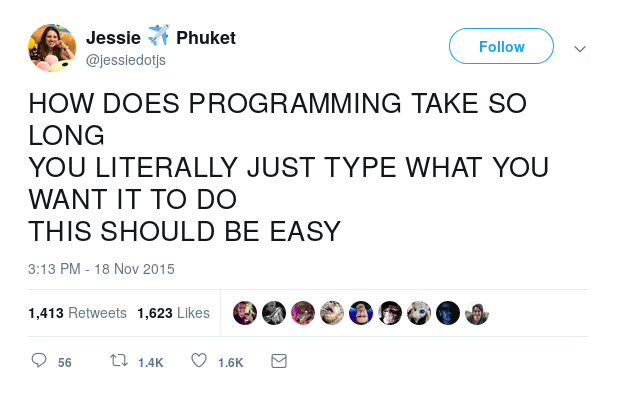
\includegraphics[width=0.8\textwidth]{tweet.png}

  {\small\url{https://twitter.com/jessiedotjs/status/667118579075141632}}
\end{frame}

\begin{frame}
  {From the birth of programming...}

  \begin{quotation}
    By June 1949 people had begun to realize that it was not so easy
    to get programs right as at one time appeared. I well remember
    when this realization first came on me with full force.

    ...
  \end{quotation}
\end{frame}

\begin{frame}
  {From the birth of programming...}

  \begin{quotation}
    ...

    The EDSAC was on the top floor of the building and the
    tape-punching and editing equipment one floor below. [...] It was
    on one of my journeys between the EDSAC room and the punching
    equipment that ``hesitating at the angles of stairs'' the
    realization came over me with full force that a \rhighlight{good
      part of the remainder of my life was going to be spent in
      finding errors in my own programs.}
  \end{quotation}
  Maurice Wilkes\\
  Memoirs of a Computer Pioneer, MIT Press, 1985, p. 145.

  \sidenote{The EDSAC was an early ``stored program''
    computers, and first ran in May 1949}
\end{frame}

\begin{frame}
  {Validation and Verification}

  The two big questions for any software system:

  \bigskip

  \begin{enumerate}
  \item {\bf Validation}: Are we building the right thing?
  \item {\bf Verification}: Are we building the thing right?
  \end{enumerate}
\end{frame}

\begin{frame}
  {Validation: What should it do?}

  A question answered by interaction with stakeholders:
  \begin{itemize}
  \item Users
  \item Purchasers \quad \textcolor{black!60}{(not necessarily the users!)}
  \item Data subjects \quad \textcolor{black!60}{(may not be the above!)}
  \item Regulatory bodies \quad \textcolor{black!60}{(e.g., ICO)}
  \item Maintaince and deployment engineers
  \item ...
  \end{itemize}

  \pause
  \bigskip

  Validation is hard, and beyond the scope of this course.
\end{frame}

\begin{frame}
  {Verification: Are we doing it right?}

  Answered by examining the system and the way it is built:

  \bigskip

  \begin{itemize}
  \item Good coding practices
  \item Code review
  \item Testing
  \item Constructing arguments, formally or informally
  \end{itemize}
\end{frame}

\begin{frame}
  {Specification}

  Validation \& Verification meet at {\bf Specification}.

  \bigskip

  A {\bf Specification} is the description of what the system ought
  and ought not to do.

  \bigskip
  \pause

  Validation : what is the specification? \\
  Verification : do we meet the specification?
\end{frame}

\begin{frame}
  {Specifying a Game}

  Technical specifications:

  \bigskip

  Must work on platform X, Y, ...
  \begin{itemize}
  \item<2-> Must work on platform X last updated in 2010, ...
  \item<3-> Must work with version 1.0.23.92 of library Z, because we won't pay for the newer one
  \end{itemize}

  \pause
  \pause
  \pause
  \bigskip

  Must have framerate of over 60fps.
\end{frame}

\begin{frame}
  {Specifying a Game}

  Feature specifications:

  \begin{enumerate}
  \item Must allow online multiplayer
  \item Must not leak personal user data when online
  \item Must have screenshot feature
  \item Must have player chat
  \item Must have blocking feature
  \end{enumerate}
\end{frame}

\begin{frame}
  {Specifying a Game}

  ``Obvious things''

  \begin{enumerate}
  \item Must not crash
  \item Must be installable
  \item When controls say ``go foward'', player's character goes forward
    \begin{enumerate}
    \item Unless there is an obstacle
    \item Or the player is frozen
    \item ...
    \end{enumerate}
  \item ...
  \end{enumerate}
\end{frame}

\begin{frame}
  {Specifying a Game}

  \begin{enumerate}
  \item Makes player feel happy
  \item Makes player feel slightly frustrated, but the good kind of frustrated, not the bad one...
  \item Player must not get stuck behind fences
  \item Game must be solvable
  \item Game must get U rating
  \item ...
  \end{enumerate}
\end{frame}

\begin{frame}
  {Real Specifications}

  Specifying complete systems is {\bf hard}.

  \bigskip

  Real-world requirements are:
  \begin{itemize}
  \item Fuzzy \quad \textcolor{black!60}{(the game must be “fun”)}
  \item Involve other systems \quad \textcolor{black!60}{(e.g., the OS, the Internet)}
  \item Involve people / physical reality
  \item Generally very complex
  \end{itemize}
\end{frame}

\begin{frame}
  {Formal Specifications}

  Nevertheless, written down specification is important:

  \bigskip

  \begin{itemize}
  \item To communicate clearly with other engineers and with stakeholders
  \item To expose conflicting requirements and ambiguity
  \item To enable formal argumentation
  \end{itemize}
\end{frame}

\weeksection{Formal Specification and Verification}

\begin{frame}
  {Formal Methods}

  The dream:

  \bigskip

  \begin{enumerate}
  \item Stakeholders get together, come to agreement, and write down a
    clear, complete, and unambiguous specification $P$;
  \item Implementors are given $P$ and produce an implementation $C$;
  \item Implementation $C$ is verified against $P$, formally, using proof.
  \item Software is perfect. Everyone is happy.
  \end{enumerate}
\end{frame}

\begin{frame}
  {Formal Methods}

  Clearly, that is only ever going to be a dream.

  \bigskip
  \pause

  {\bf But,} we can formally specify and sometimes verify:

  \medskip

  \begin{itemize}
  \item High-value, critical, aspects of a system
  \item Low-level, unambiguous aspects of components
  \item Simple but useful properties that apply ``everywhere''
  \end{itemize}

\end{frame}

\begin{frame}
  {Formal Specifications}

  Example:

  \bigskip

  \begin{center}
    If a transaction is acknowledged by the server, then it must have
    already been logged in the journal and written to durable storage.
  \end{center}

  \bigskip

  Specifying an aspect of behaviour that is critical to the system's
  operation.
\end{frame}

\begin{frame}
  {Formal Specifications}

  Example:

  \bigskip

  \begin{center}
    This function must sort the input array in ascending order.
  \end{center}

  \bigskip

  Specifying a (relatively) low-level aspect of part of a system that
  other parts rely on.
\end{frame}

\begin{frame}
  {Formal Specifications}

  Example:

  \bigskip

  \begin{center}
    If a function's type says it returns an \texttt{int}, then it
    either returns an \texttt{int}, or raises an exception, or does
    not return.
  \end{center}

  \bigskip

  An example of a specification written in the type system of a
  language, and enforced by the language implementation.
\end{frame}

\begin{frame}
  {Logical Specifications}

  Formal logic can be used to write down a specification of a system,
  assuming {\bf we have a formal model of how the system operates}.

  \bigskip
  \pause

  So the problem becomes:
  \begin{enumerate}
  \item Fix a formal model of how the system operates
  \item Prove the formal model meets the specification
  \end{enumerate}

\end{frame}

\begin{frame}
  {Formal Models of Programs}

  \begin{enumerate}
  \item As functions, with behaviour specified by equations.

    This is what you did in \texttt{ask} in CS106.

    \bigskip
  \item As logical proofs themselves, following the ``evidence''
    interpretation. See CS410.

    \bigskip
  \item Modelled as predicates in the logic.

    We will do this here.

    \bigskip
  \item Many others...
  \end{enumerate}
\end{frame}

\begin{frame}
  {A Simple Formal Model}

  A simple formal model of program execution can be defined in terms
  of a single predicate:
  \begin{displaymath}
    \mathrm{exec}(\mathit{prog}, \mathit{initState}, \mathit{finalState})
  \end{displaymath}
  meaning:
  \begin{itemize}
  \item the program $\mathit{prog}$,
  \item when started in initial state $\mathit{initState}$,
  \item can terminate with final state $\mathit{finalState}$.
  \end{itemize}
\end{frame}

\begin{frame}
  {A Simple Formal Model}

  We will flesh out what $\mathrm{exec}$ means by using axioms.

  \bigskip

  Even without knowing what the exact axioms are, we can make some
  general definitions.
\end{frame}

\begin{frame}
  {A Simple Formal Model}

  A program $\mathit{prog}$...

  \bigskip

  ... terminates starting in state $\mathit{s}$ if:
  \begin{displaymath}
    \exists \mathit{fs}.~\mathrm{exec}(\mathit{prog}, \mathit{s}, \mathit{fs})
  \end{displaymath}

  \bigskip

  ... terminates {\bf on all inputs} if:
  \begin{displaymath}
    \forall \mathit{s}. \exists \mathit{fs}.~\mathrm{exec}(\mathit{prog}, \mathit{s}, \mathit{fs})
  \end{displaymath}

\end{frame}

\begin{frame}
  {A Simple Formal Model}

  A program $\mathit{prog}$ ...

  \bigskip

  ... is deterministic if:
  \begin{displaymath}
    \forall s. \forall s_1. \forall s_2. \mathrm{exec}(\mathit{prog}, s, s_1) \to \mathrm{exec}(\mathit{prog}, s, s_2) \to s_1 = s_2
  \end{displaymath}

\end{frame}

% PUT THIS IN THE COURSEWORK!

% \begin{frame}
%   {A Simple Formal Model}

%   Two programs $\mathit{prog}_1$ and $\mathit{prog}_2$ are
%   \emph{equivalent} {\bf up to non-termination} if:
%   \begin{displaymath}
%     \forall s.\forall s_1.\forall s_2. \mathrm{exec}(\mathit{prog}_1, s, s_1) \to \mathrm{exec}(\mathit{prog}_2, s, s_2) \to s_1 = s_2
%   \end{displaymath}

%   \bigskip

%   They have equivalent termination behaviour if:
%   \begin{displaymath}
%     \forall s.(\exists s'. \mathrm{exec}(\mathit{prog}_1, s, s')) \leftrightarrow (\exists s'. \mathrm{exec}(\mathit{prog}_2, s, s'))
%   \end{displaymath}
%   Note: $P \leftrightarrow Q$ is shorthand for $(P \to Q) \land (Q \to P)$.
% \end{frame}

\begin{frame}
  {A Simple Formal Model}

  This model is \emph{very} simple.

  \bigskip

  It does not include:
  \begin{enumerate}
  \item Resources, such as amount of time required
  \item Interactive computation, input is provided all at once
  \item Online computation, output is provided all at once
  \item Errors or exceptions distinct from states
  \end{enumerate}
\end{frame}

\begin{frame}
  {A Simple Formal Model}

  However, it is useful:

  \bigskip

  \begin{enumerate}
  \item \emph{Partial} and \emph{non-deterministic} computation
  \item Programs and data can be mixed
  \item Enough to talk about specifications
  \end{enumerate}
\end{frame}

\weeksection{Hoare Logic}

\begin{frame}
  {Specifying Programs' Behaviour}

  The classic specification of a program's behaviour:

  \bigskip

  \begin{enumerate}
  \item If the initial state $s_1$ satisfies some predicate $P(s_1)$; and
  \item the program starts in state $s_1$ and finishes in state $s_2$, then
  \item the final state $s_2$ satisfies a predicate $Q(s_2)$.
  \end{enumerate}

  \bigskip

  $P$ is the \emph{precondition}; $Q$ is the \emph{postcondition}.
\end{frame}

\begin{frame}
  {Hoare Triples}

  This is often written like this:
  \begin{displaymath}
    \{ P \}\, \mathit{prog}\, \{ Q \}
  \end{displaymath}
  which is called a \emph{Hoare triple}.

  \bigskip

  The formal definition is:
  \begin{displaymath}
    \forall s_1. \forall s_2. P(s_1) \to \mathrm{exec}(\mathit{prog},s_1,s_2) \to Q(s_2)
  \end{displaymath}
  If $P$ is true before executing $\mathit{prog}$, then $Q$ is true afterwards.
\end{frame}

\begin{frame}
  {Hoare Triples}

  Hoare triples
  \begin{displaymath}
    \{ P \}\, \mathit{prog}\, \{ Q \}
  \end{displaymath}
  specify \emph{partial} correctness.

  \bigskip

  Only says \emph{if the program finishes}, then the postcondition $Q$ holds.

  \bigskip

  \emph{Total} correctness will be defined later...
\end{frame}

\begin{frame}
  {Hoare Logic}

  \emph{Hoare Logic} is a deductive system for judgements of the form:
  \begin{displaymath}
    \{ P \}\, \mathit{prog}\, \{ Q \}
  \end{displaymath}

  \bigskip

  The ``Big idea'' is that (mostly) the structure of the proof follows
  the structure of the program.

  % \bigskip

  % Topic 6 will use a specific tool for Hoare Logic.
\end{frame}

% \begin{frame}
%   {A Simple Programming Language}

%   \begin{displaymath}

%   \end{displaymath}
% \end{frame}

\begin{frame}
  {Hoare Logic: Rules}

  Let $\mathrm{skip}()$ be the program that does nothing, successfully.

  \bigskip

  Its rule:
  \begin{displaymath}
    \inferrule* [right=Skip]
    { }
    {\{ P \}\, \mathrm{skip}()\, \{ P \}}
  \end{displaymath}

  \bigskip

  $\mathrm{skip}()$ doesn't alter the state: whatever was true before is true after.
\end{frame}

\begin{frame}
  {Hoare Logic: Rules}

  Let $\mathrm{seq}(p_1,p_2)$ be the program that first does $p_1$ then does $p_2$.

  \bigskip

  Its rule:
  \begin{displaymath}
    \inferrule* [right=Seq]
    {\{ P \}\,p_1\,\{ R \} \\ \{ R \}\,p_2\,\{ Q \}}
    {\{ P \}\,\mathrm{seq}(p_1,p_2)\,\{ Q \}}
  \end{displaymath}

  \bigskip

  If $p_1$ gets us from $P$ to $R$, and $p_2$ gets us from $R$ to $Q$,
  then doing them in sequence gets us from $P$ to $Q$.
\end{frame}

\begin{frame}
  {Hoare Logic: Rules}

  Let $\mathsf{doUpdate}(s)$ be some function on states, and
  $\mathrm{update}$ be the \emph{program} that performs that update.

  \bigskip

  There are two rules, depending on whether we are reasoning
  ``forwards'' or ``backwards''.
\end{frame}

\begin{frame}
  {Hoare Logic: Rules}

  Rule, variant 1 (\emph{weakest precondition}):
  \begin{displaymath}
    \inferrule* [right=Update-Bwd]
    { }
    {\{ P[s := \mathsf{doUpdate}(s)] \}\,\mathrm{update}()\,\{ P \}}
  \end{displaymath}

  \bigskip

  Rule, variant 2 (\emph{strongest postcondition}):
  \begin{displaymath}
    \inferrule* [right=Update-Fwd]
    { }
    {\{ P \}\,\mathrm{update}()\,\{ \exists s'. s = \mathsf{doUpdate}(s') \land P[s := s'] \}}
  \end{displaymath}
\end{frame}

\begin{frame}
  {Hoare Logic: Rules}

  Let $\mathrm{ifC}(p_1,p_2)$ be the program that runs $p_1$ if $C$ is true, and $p_2$ if $C$ is not true.

  \bigskip

  \begin{displaymath}
    \inferrule* [right=If]
    {\{ C \land P \}\,p_1\,\{ Q \} \\ \{ \lnot C \land P \}\,p_2\,\{ Q \}}
    {\{ P \}\,\mathrm{ifC}(p_1,p_2)\,\{ Q \}}
  \end{displaymath}
\end{frame}

\begin{frame}
  {Hoare Logic: Rules}

  Let $\mathrm{whileC}(p)$ be the program that runs $p$ until condition $C$ is false.

  \bigskip

  \begin{displaymath}
    \inferrule* [right=While]
    {\{ C \land P \}\,p\,\{ P \}}
    {\{ P \}\,\mathrm{whileC}(p)\,\{ \lnot C \land P \}}
  \end{displaymath}

  \bigskip

  In this case, $P$ is the \emph{loop invariant}.
\end{frame}

\begin{frame}
  {Hoare Logic: Rules}

  Consequence:
  \begin{displaymath}
    \inferrule* [right=Consequence]
    {P' \vdash P \\ \{ P \}\,p\,\{ Q \} \\ Q \vdash Q'}
    {\{ P' \}\,p\,\{ Q' \}}
  \end{displaymath}

  \bigskip
  \begin{enumerate}
  \item \emph{Strengthen} the precondition: $P' \vdash P$
  \item \emph{Weaken} the postcondition: $Q \vdash Q'$
  \end{enumerate}
\end{frame}

\begin{frame}
  {Hoare Logic}

  Each of these rules can be proved sound with respect to the partial
  correctness property:
  \begin{displaymath}
    \forall s_1. \forall s_2. P(s_1) \to \mathrm{exec}(\mathit{prog},s_1,s_2) \to Q(s_2)
  \end{displaymath}

  \bigskip

  We need to assume some axioms for each of the different program
  constructs; this is our {\bf trusted base}. If we get these axioms
  wrong, then a proof in Hoare logic means nothing.

%  See the online notes for the proofs.
\end{frame}

\begin{frame}
  {Hoare Logic: A Quirk}

  If $C$ is the condition that is always true, then the program
  \begin{displaymath}
    \mathrm{whileC}(\mathrm{skip}())
  \end{displaymath}
  satisfies \emph{any} specification:
  \begin{displaymath}
    \{ P \}\,\mathrm{whileC}(\mathrm{skip}())\,\{ Q \}
  \end{displaymath}
  Why?
\end{frame}

\begin{frame}
  {Total Correctness}

  Total correctness is usually written as:
  \begin{displaymath}
    [ P ]\,\mathit{prog}\,[ Q ]
  \end{displaymath}
  and is defined as:
  \begin{displaymath}
    \forall s_1. P(s_1) \to (\exists s_2. \mathrm{exec}(\mathit{prog},s_1,s_2) \land Q(s_2))
  \end{displaymath}

  \bigskip

  All of the rules are the same as for the partial version, except for
  the rule for $\mathrm{whileC}(p)$.
\end{frame}

\begin{frame}
  {Summary}

  \begin{itemize}
  \item Formal Specification and Verification require a formal model
  \item The execution predicate is a simple but useful model
  \item Hoare logic is a deductive system for proving programs satisfy specifications in this model
  \item It comes in partial and total variants.
  \end{itemize}
\end{frame}


% \begin{frame}
%   {What makes Programming Hard?}

%   \begin{enumerate}
%   \item Getting the syntax right? \\
%     \sidenote{basically not a problem; loads of IDE support}

%     \bigskip
%   \item Needing Fancy Algorithms? \\
%     \sidenote{Relatively rare to have to do something completely new}

%     \bigskip
%   \item Making sure it does the right thing? \\
%     \sidenote{Validating the \emph{specification}}

%     \bigskip
%   \item Making sure you do it right? \\
%     \sidenote{\emph{Verifying} the program against the Specification}
%   \end{enumerate}
% \end{frame}

% \begin{frame}
%   {Current best practice}

%   \sidenote{An uncharitable caricature}

%   \bigskip

%   \begin{enumerate}
%   \item Write or alter some code
%   \item Test it
%     % \sidenote{usually on a fixed set of test cases}\\
%     % \sidenote{often written by the same person who wrote the code}
%   \item Release it
%   \item Users find bugs, or tell you that's not what they wanted
%   \item Goto step 1
%   \end{enumerate}

%   \bigskip

%   You can rearrange the \sout{deckchairs} steps and call it Agile, or
%   TDD, or Waterfall, or eXtreme Programming, or whatever.
% \end{frame}

% \begin{frame}
%   {Specification}

%   Implicit in the previous is the existence of some
%   \emph{specification}.

%   \bigskip

%   Crude idea: there is a specification that tells us everything about what a program must do

%   Better idea: there are overlapping specifications of different levels of detail covering different aspects of the system:
%   \begin{enumerate}
%   \item High level requirements: produces the ``right'' reports
%   \item ``Non-functional'': performance
%   \item ``Non-functional'': easy to use
%   \item ``Non-functional'': is ``fun''
%   \item Low-level: doesn't crash, if a function says it returns an
%     integer, then it actually does, if a method says it sorts arrays
%     then it actually sorts arrays, ...
%   \end{enumerate}
% \end{frame}

% \begin{frame}
%   {Can we Verify programs?}

%   Given a program \texttt{C} and a specification $P$, can we:
%   \begin{enumerate}
%   \item Verify that \texttt{C} satisfies $P$...
%   \item \emph{rigorously}...
%   \item with \emph{no room for doubt}...
%   \item \emph{easily}, \emph{cost effectively}, \emph{maintainably}...
%   \end{enumerate}
% \end{frame}

% \begin{frame}
%   {No}

%   \begin{enumerate}
%   \item Writing specifications is hard -- what should the code do? \\
%     \sidenote{probably the hardest bit}\\
% %    \sidenote{I really hate this damn machine / I wish that they would sell it \\ \quad\quad\quad It never does quite what I want / But only what I tell it}
%   \item We always have to make assumptions (contra point 3) \\
%     \sidenote{assume things about the OS, the hardware, the universe etc.}
%   \item Programs are very, very big and complex \\
%     \sidenote{and the proofs are often very boring}
%   \item Currently, proving programs is time consuming and difficult.
%   \end{enumerate}
% \end{frame}

% \begin{frame}
%   \sechead{Nevertheless...}

%   We're going to try. \\
%   \sidenote{and we might learn something on the way...}
% \end{frame}



% \begin{frame}
%   {Specifying Programs}

%   Ways of specifying what programs do:
%   \begin{enumerate}
%   \item As equations (as in Ask)
%   \item As it is done in Syrup, by a reference implementation
%   \item Pre- and post-conditions
%   \item Traces
%   \item ...
%   \end{enumerate}
% \end{frame}

% \begin{frame}
%   {Pre- and Post-conditions}


% \end{frame}

% \begin{frame}
%   {An Execution Predicate}
% \end{frame}

% \weeksection{Program Verification}

% \weeksection{}

\end{document}
